\documentclass[a4paper,10pt,parskip=half]{scrartcl}

\usepackage[usenames,dvipsnames]{xcolor}
\usepackage{graphicx}
\usepackage[utf8]{inputenc} %-- pour utiliser des accents en français
\usepackage{mathpazo}
\usepackage{amsmath,amssymb,amsthm} 
\usepackage[round]{natbib}
\usepackage{url}
\usepackage{xspace}
\usepackage{multirow}
\usepackage[left=20mm,top=20mm]{geometry}
\usepackage[ruled,vlined,linesnumbered]{algorithm2e}
\usepackage{subcaption}
\usepackage{booktabs}
\usepackage{colortbl}
\usepackage{hyperref}
\usepackage{boxedminipage}
\usepackage{fontawesome}
\usepackage{lastpage}
\usepackage{todonotes}
\usepackage{listings}
\usepackage{ccicons}
\usepackage{float}
\usepackage{tikz}
\usepackage[tikz]{mdframed}


\usepackage[autooneside,headsepline]{scrlayer-scrpage}
\clearpairofpagestyles
\ihead*{GEO1004.2020}
% \ohead*{Lesson 01}
% \setheadsepline{0.5pt}
\KOMAoptions{footsepline=:.25\textwidth,clines}
\cfoot{\pagemark\ of \pageref{LastPage}}


\newcommand{\ie}{ie}
\newcommand{\eg}{eg}
\newcommand{\reffig}[1]{Figure~\ref{#1}}
\newcommand{\refsec}[1]{Section~\ref{#1}}
\newcommand{\refeq}[1]{Equation~\ref{#1}}

\setcapindent{1em} %-- for captions of Figures


\renewcommand{\refname}{References \& further reading}
\renewcommand{\contentsname}{\vspace{-15mm}}

\definecolor{light-gray}{gray}{0.97}
\definecolor{myred}{RGB}{111,12,31}
\definecolor{mygreen}{RGB}{35,138,35}

\newfloat{myfloat}{thp}{lop}

\newmdenv[%
  outerlinewidth=1.5,%
  roundcorner=5pt,%
  linecolor=myred,%
  backgroundcolor=light-gray,%
  frametitle=\faExternalLink\ To read or watch,
]{link-box}

\newmdenv[%
  outerlinewidth=1.5,%
  roundcorner=5pt,%
  linecolor=mygreen,%
  backgroundcolor=light-gray,%
  frametitle=\faCog\ How does it work in practice?,
]{practice-box}

\newcommand{\lessonNumber}{Lesson 2.1}

\newcommand{\Orient}{O\textsc{rient}\xspace}
\newcommand{\Insphere}{I\textsc{n}S\textsc{phere}\xspace}


\newtheorem{definition}{Definition}



\title{3D building reconstruction}

\ohead*{\lessonNumber}
\titlehead{\thispagestyle{headings}}
\author{\lessonNumber\footnote{\ccbysa\ Ravi Peters. This work is licensed under a Creative Commons Attribution 4.0 International License (\url{http://creativecommons.org/licenses/by/4.0/})\newline(last update: \today)}}
\date{}
\begin{document}
\pagestyle{scrheadings}

\maketitle

\noindent\rule{5cm}{0.4pt}
\tableofcontents
\noindent\rule{5cm}{0.4pt}
\vspace{5mm}

%\newpage
In the previous lesson we discussed how to model 3D objects using the boundary representation.
You learned about data structures to represent the geometry and topology of a 3D object's surface in a very structured and organised way.
In this lesson we will look at how you could create such a structured representation from a much less structured form of 3D geoinformation, namely a point cloud.

In automatic building reconstruction we aim to construct 3D mesh models for individual buildings from some form of elevation measurements, \ie\ a raster-based DSM or a point cloud, without any manual interventions (see Figure~\ref{fig:bk-building-recon}).
\begin{figure}
	\centering
	\begin{subfigure}[b]{0.45\linewidth}
		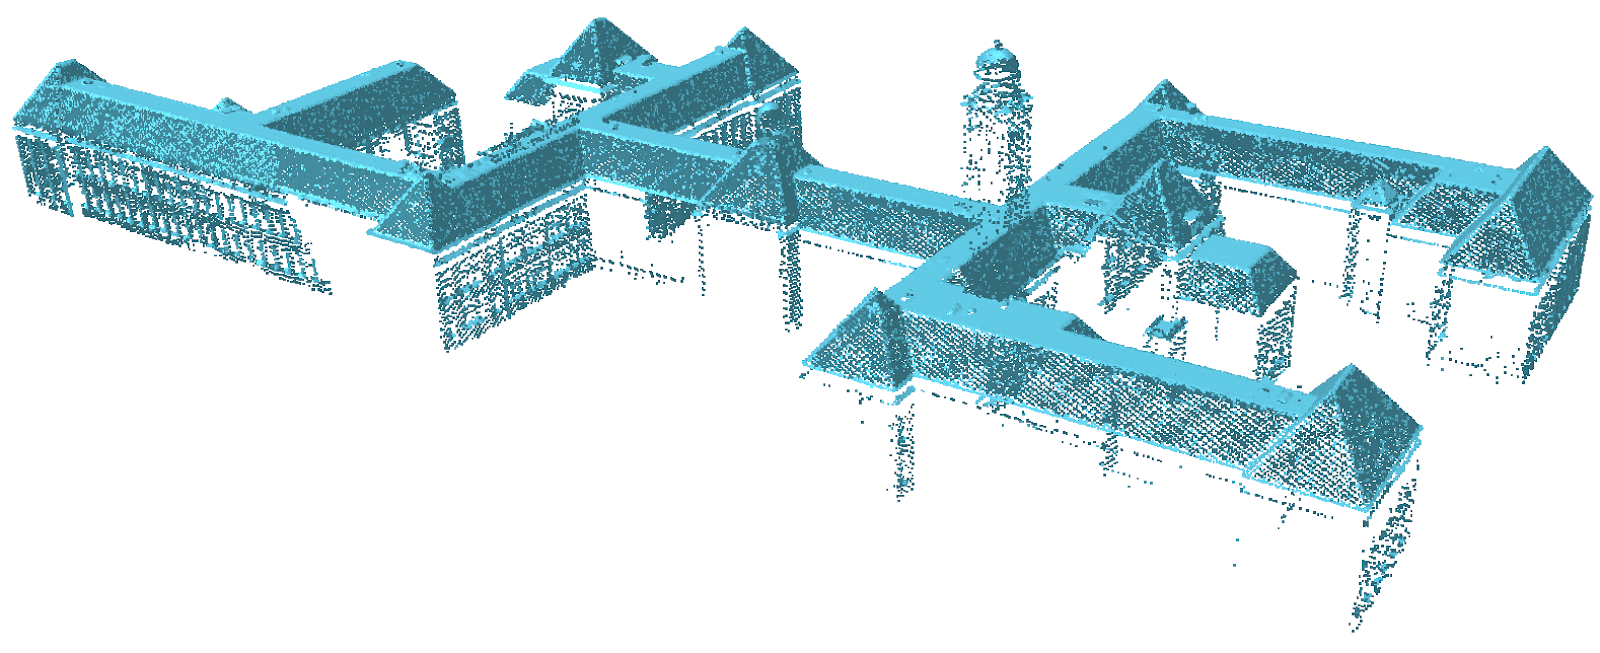
\includegraphics[width=\linewidth]{figs/bk-pointcloud.png}
		\caption{Point cloud}%
		\label{subfig:bk-pc}
	\end{subfigure}
	\quad
	\begin{subfigure}[b]{0.45\linewidth}
		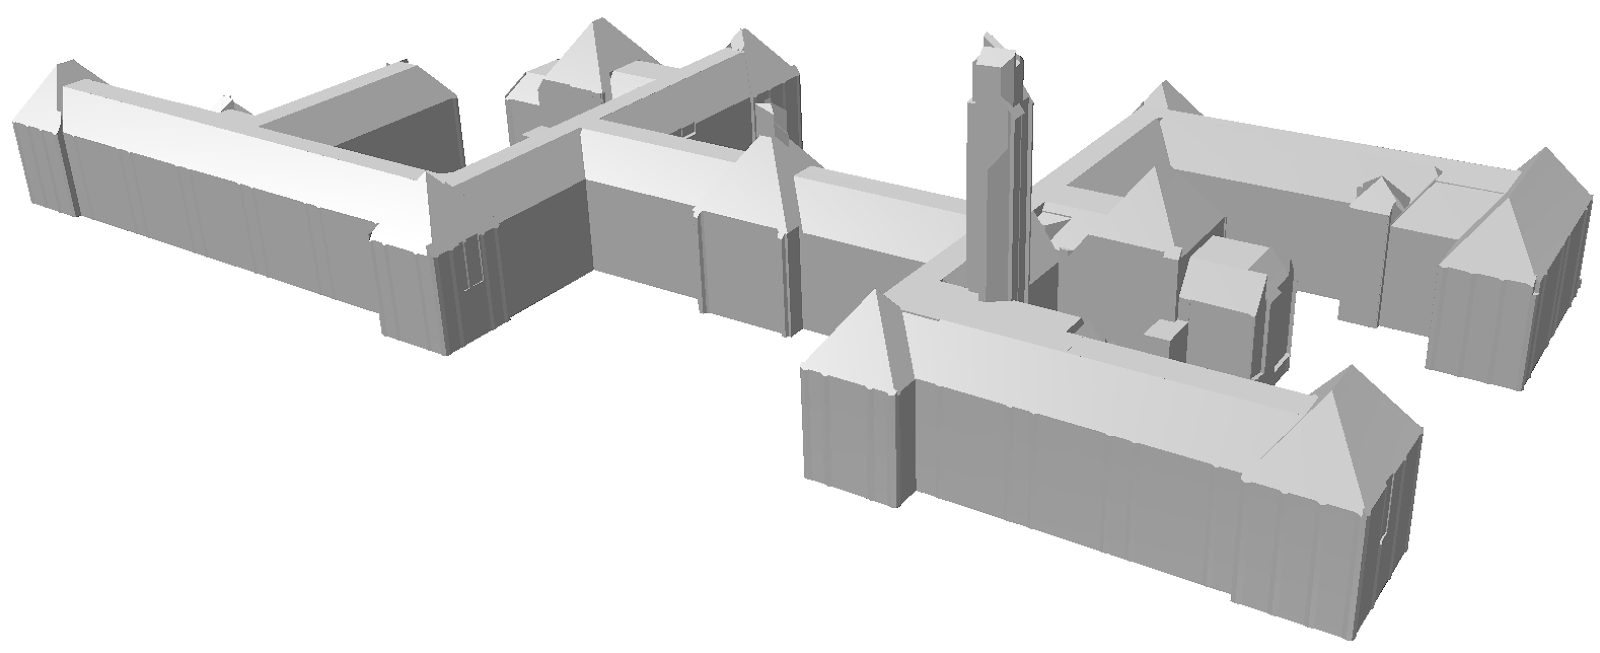
\includegraphics[width=\linewidth]{figs/bk-mesh.png}
		\caption{Mesh model}%
		\label{subfig:bk-mesh}
	\end{subfigure}
	\caption{Building reconstruction transforms a point cloud into a mesh model.}%
	\label{fig:bk-building-recon}
\end{figure}
It can be considered as one step in the geoinformation chain, since we essentially transform 'raw' and unorganised point measurements into more structured and semantically rich 3D models.
Compared to a point cloud, such models are much more useful for applications such as environmental simulations of wind, air pollution, and noise propagation, but also building energy demand estimation and urban planning in general.
Many of these applications require knowledge about the volume or surface area of a building, or the distinction between the interior and exterior of a building, which is evidently much easier to derive from a mesh with a clearly defined boundary than from a point cloud.
In addition, meshes are typically more compact which makes them more efficient to store and process.

This is not to say that meshes are always superior to point clouds. 
For example some of the finer details that may be present in a point cloud could be lost in the mesh representation. 
Furthermore, there is always the risk of introducing new errors and deviations from the original measurement in the building reconstruction process. 
But ultimately, the many benefits of representing a building as a mesh outweigh these disadvantages for many applications.

In this lesson we will first list common challenges and requirements for the building models that are to be constructed. Second, we will look at the important engineering choices in designing a building reconstruction algorithm. And finally, we will discuss one particular approach that was designed to work on Dutch open data in more detail.

%%%
%
\section{Building model requirements and reconstruction challenges}
When designing a building reconstruction method, it is important to carefully consider both the \emph{model requirements} and the \emph{reconstruction challenges}. 
The model requirements specify in detail what properties a reconstructed building model should have. 
Model requirements are mostly application dependent.
For example, an application that performs heavy geometric processing on the building models has stricter geometry and topology requirements than an application that merely visualises the building models.
Reconstruction challenges, on the other hand, are mostly input dependent. 
It is about the characteristics of the input data and the typical shape of the buildings that are present in the input data.
Simply put, it is relatively easy to design a reconstruction approach for a very high quality point cloud that contains only very simple building shapes, whereas reconstructing complex building shapes from a very sparse and low quality input point cloud is substantially more difficult.

\subsection{Building model requirements}
%Following are some of the commonly encountered building model requirements.
%An ideal reconstruction method would satisfy all these requirement, but note that in practice we often encounter models that fail in one or several of these.

\begin{description}
	\item[Low complexity] Means that the building model ought to have as few vertices, edges, and faces as possible. Building models with a low complexity are faster to process and take up less storage space.
	\item[Good data fit] The surfaces of the building model should have the lowest possible error with respect to the input point cloud. This error can be measured as the root mean square of all the shortest distances from each input point to the model surface. 
	\item[Watertight] Implies that the surface of the building model has no creaks and holes. In other words, if one would `fill' the model with water it can not leak out anywhere. This is important for volume computations for example. 
	\item[2-manifold] As explained in the previous lesson. A 2-manifold surface is by definition also watertight. In addition it guarantees that the model has no dangling edges or isolated vertices and that 2D topological data structures can be used to represent it.
	\item[ISO19107 compliant] Validity according to the ISO19107 standard, means---among other things---that the mesh has consistently oriented faces, no duplicated vertices, and no self intersecting geometries. This makes the model generally easier to process since many assumptions can be made about the structure of the mesh. Lesson 5.2 discusses the ISO19107 standard in detail.
	\item[Level of Detail (LoD)] Specifies the degree of generalisation in the roof structure of the reconstructed building model when compared to how the actual building is built. An LoD 1 model for example only allows horizontal flat roof surfaces (even if the actual building roof looks different), whereas an LoD 2 model also allows for more detailed multi-pitched roof shapes. For the remainder of this lesson we will focus on LoD 2 models. Lesson 6.1 discusses the possible LoDs for building models in more detail.
\end{description}

\subsection{Reconstruction challenges}

\begin{description}
	\item[Variation in architectural styles] Urban environments can be complex and organised with a high degree of randomness due to their anarchical creation over time. This makes it difficult to design a reconstruction algorithm that is able to model 100\% of the buildings on earth. It is probable that there are always a few cases that violate some of the assumptions made in the building reconstruction method. For example, to simplify a reconstruction approach, it may seem reasonable to assume that buildings are not built on top of each other without touching each other. And while this assumption is valid in more than 99\% of the cases, in practice there are some violations of this assumption (see Figure~\ref{fig:debrug}).
	\begin{figure}
		\centering
		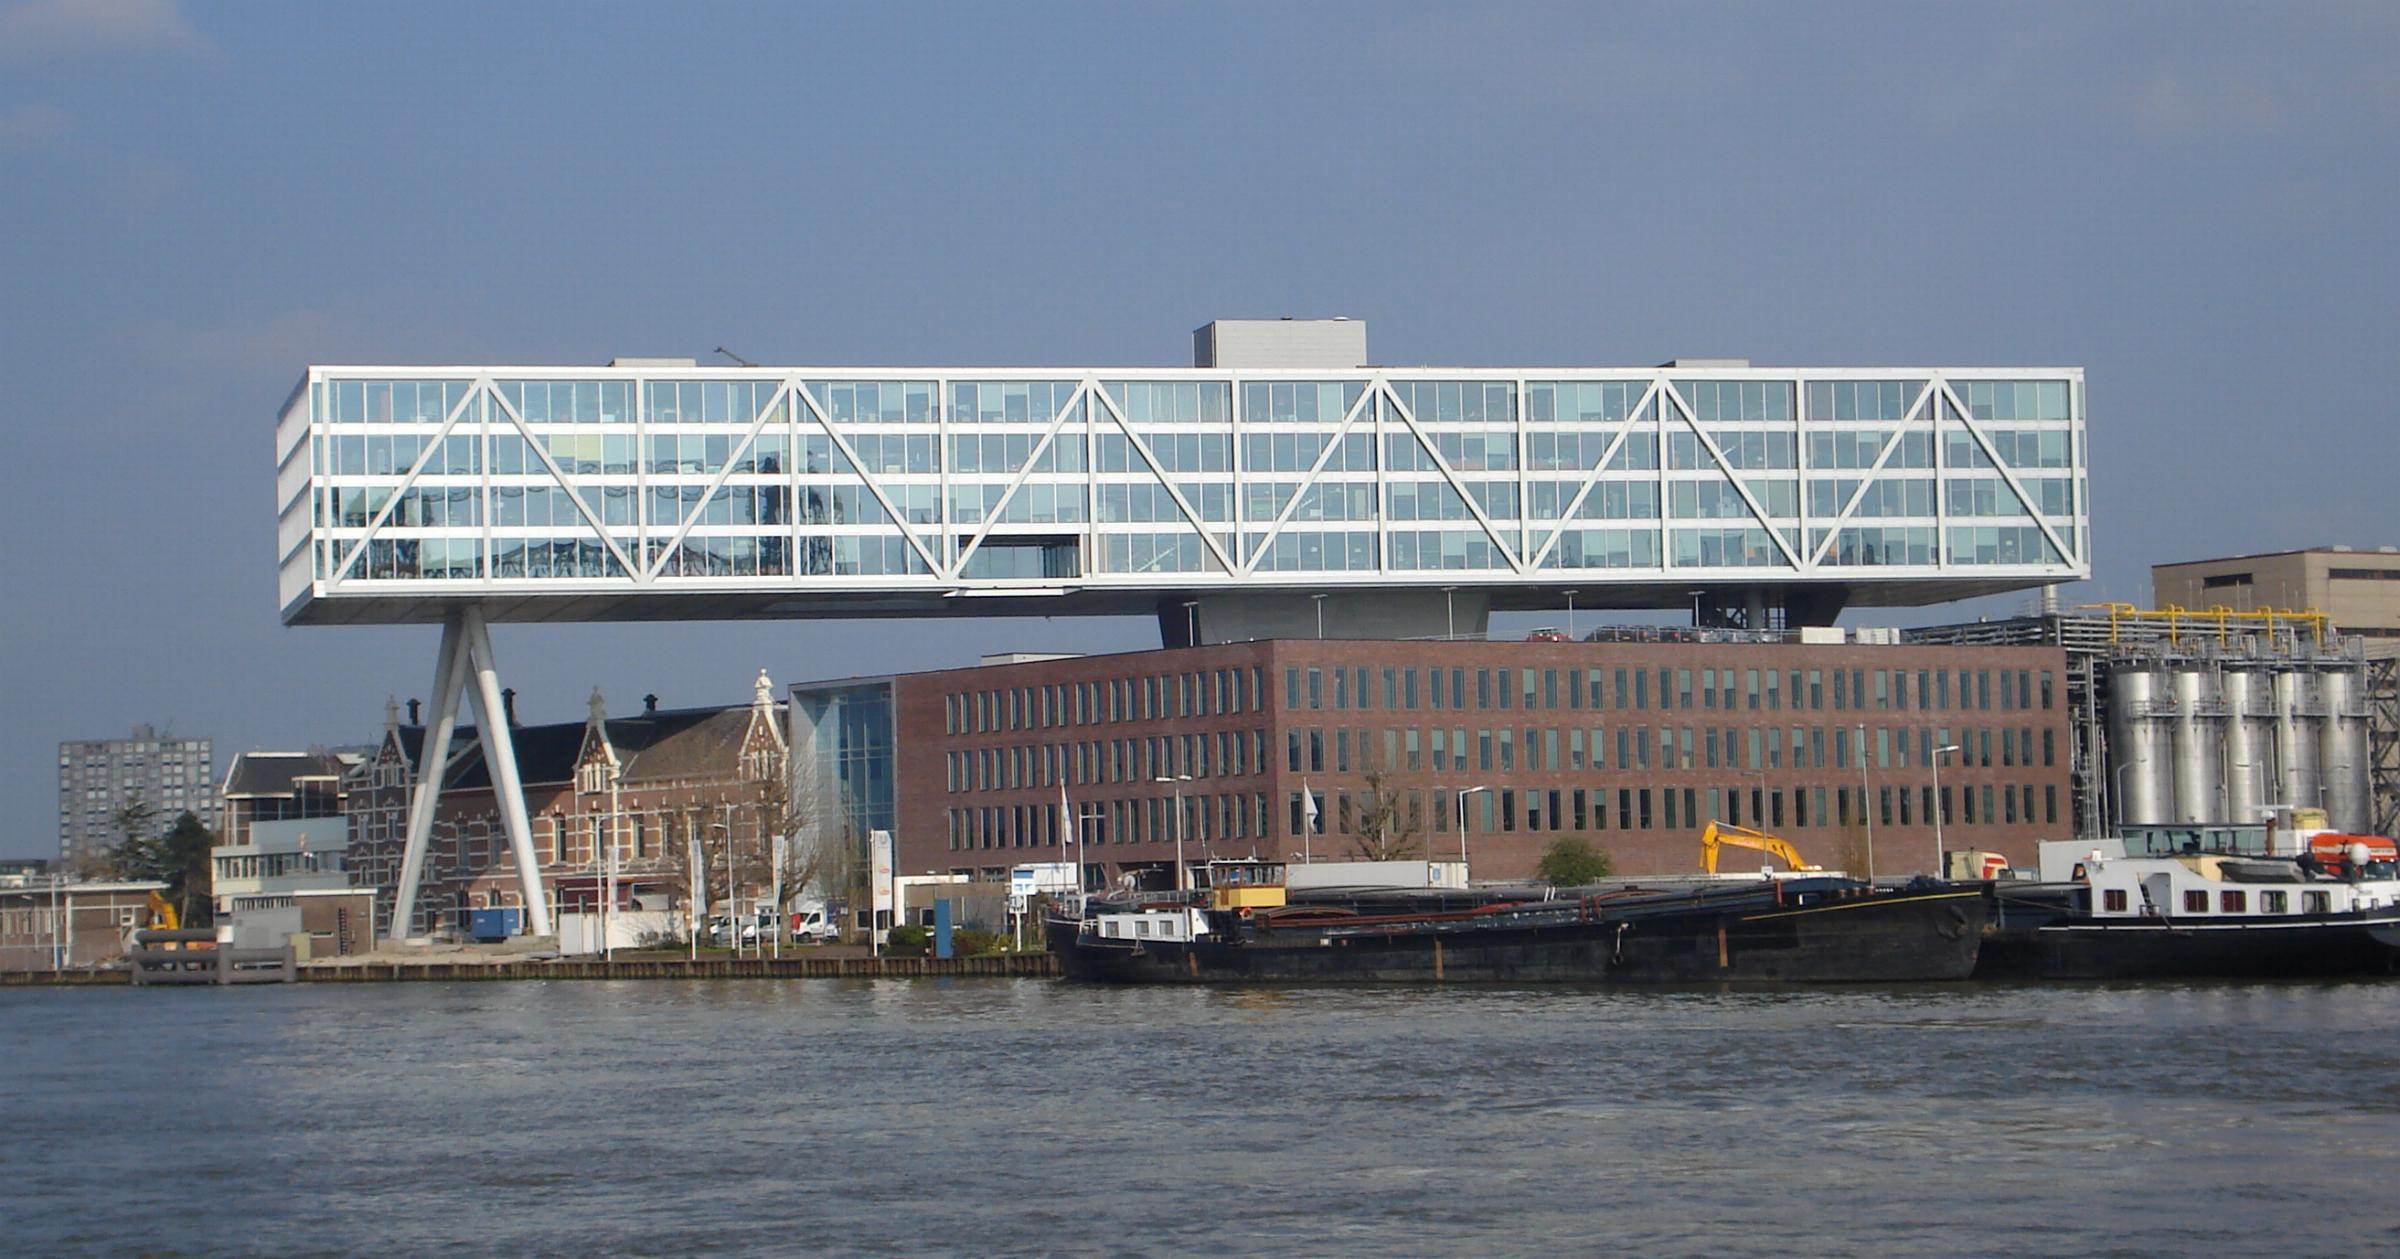
\includegraphics[width=0.8\linewidth]{figs/de_brug.jpg}
		\caption{A complex urban environment.}%
		\label{fig:debrug}
	\end{figure}
	
	\item[Quality and completeness of the input data] This mostly relates to how the input data, \ie\ the point cloud, was acquired (compare \eg\ Figure~\ref{fig:pc-quality:low} to \ref{fig:pc-quality:high}). Most building reconstruction methods work with point clouds that are captured from an airplane. This is the most efficient way to cover large areas, but it also means that not all the exterior surfaces of a building are captured due to occlusion. In particular facades and the underside of overhanging structures may be missing in such datasets. If a surface is missing in the point cloud we need to compensate for that with assumptions on what we expect the building to look like. For instance, we could assume that facades are always vertical so that we can simply model a vertical plane from the roofline to the ground. 
	Other point cloud properties are also important. For example the point density is indicative for the smallest details, \eg\ the smallest planar surfaces, that we can reliably detect in the point cloud. Consequently we can not reasonably expect to see smaller details in the reconstructed building model unless very strong assumptions are taken on the type of building shape that is modelled.
	\begin{figure}
		\centering
		\begin{subfigure}[b]{0.45\linewidth}
			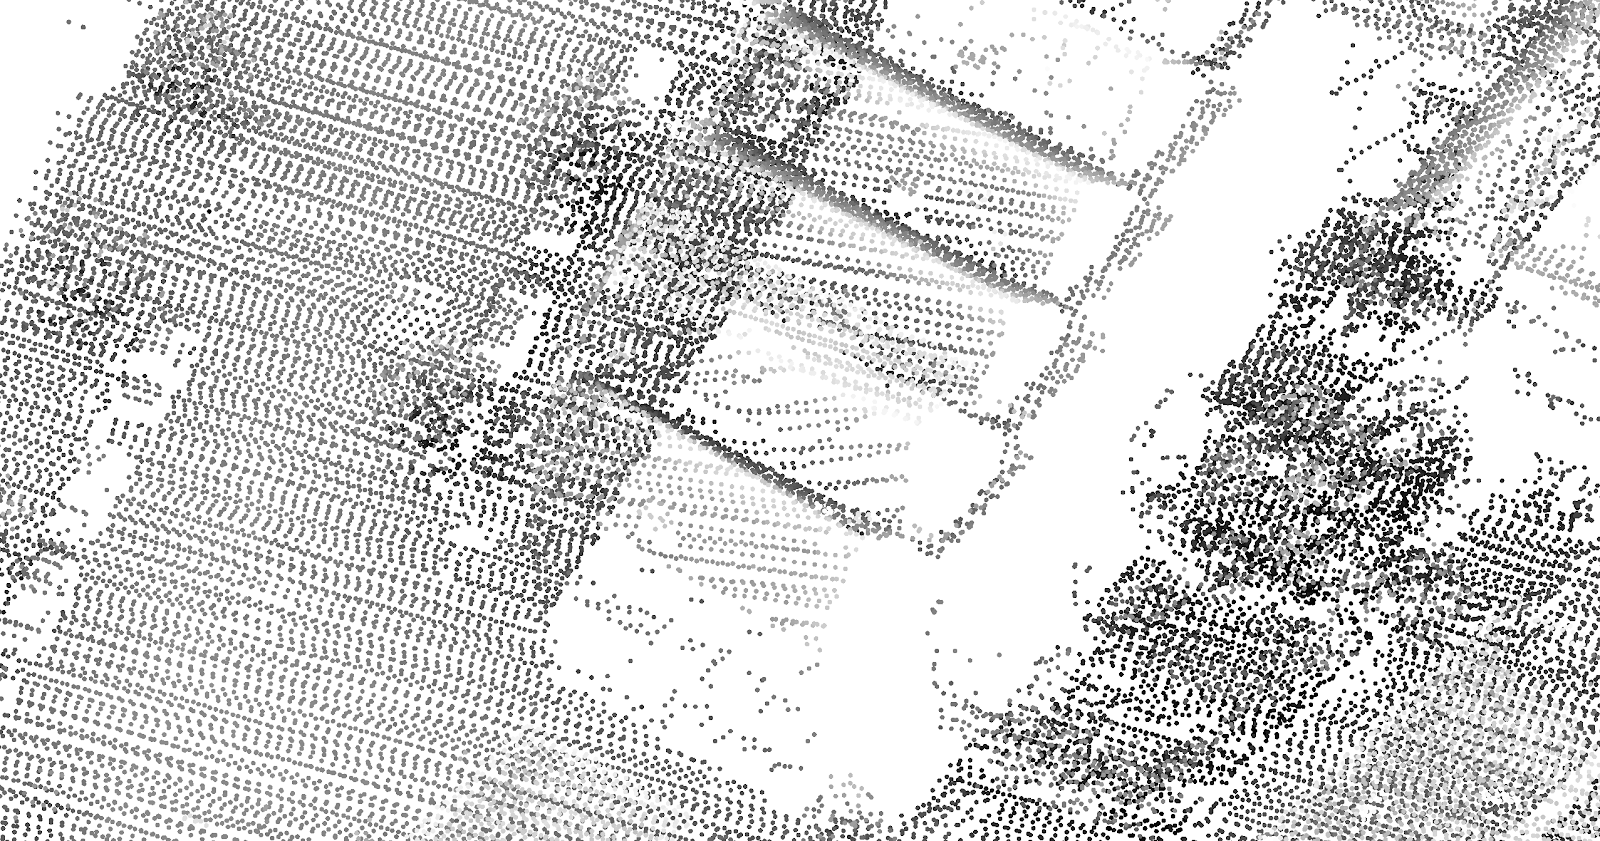
\includegraphics[width=\linewidth]{figs/rdam16_ahn2.png}
			\caption{Low point density with missing facades.}%
			\label{fig:pc-quality:low}
		\end{subfigure}
		\quad
		\begin{subfigure}[b]{0.45\linewidth}
			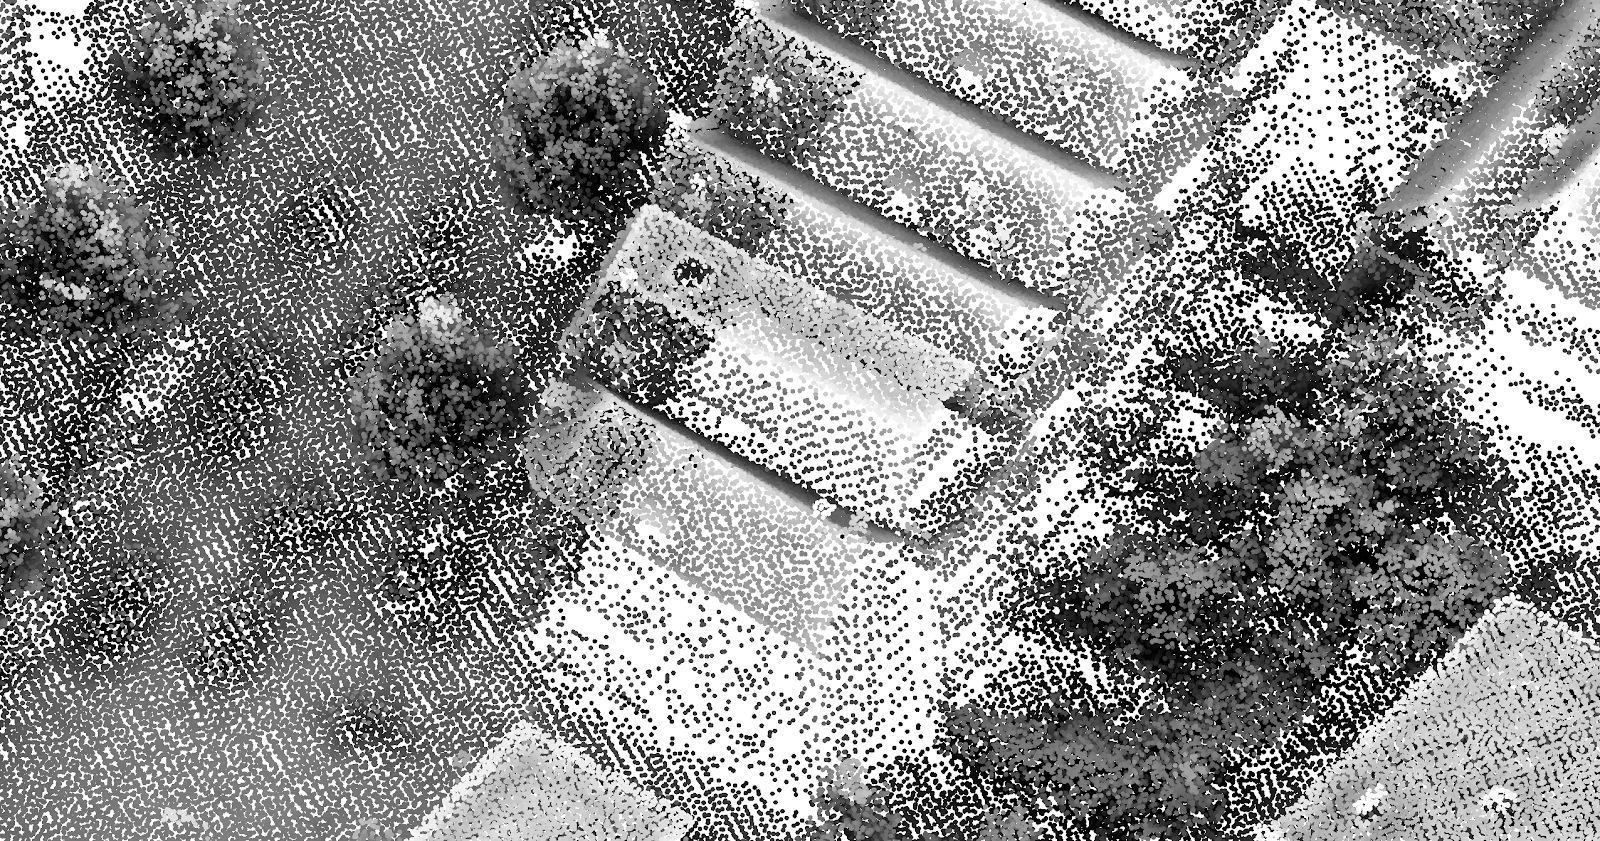
\includegraphics[width=\linewidth]{figs/rdam16_d.png}
			\caption{High point density and points on facades.}%
			\label{fig:pc-quality:high}
		\end{subfigure}
		\caption{Varying point cloud qualities.}%
		\label{fig:pc-quality}
	\end{figure}
	
\end{description}

%%%
%
\section{Data driven versus model driven building reconstruction}
Building reconstruction has been a popular topic among researcher over the last few decades. 
Many approaches exist that vary in the expected type and resolution or density of input data, the precise model requirements, and in how restricted they are to a particular architectural style.
One could classify these methods on a linear scale with on one extreme the purely so-called \emph{data  driven} approaches and on the other extreme the purely so-called \emph{model driven} approaches.
\begin{figure}
	\centering
	\begin{subfigure}[b]{0.45\linewidth}
		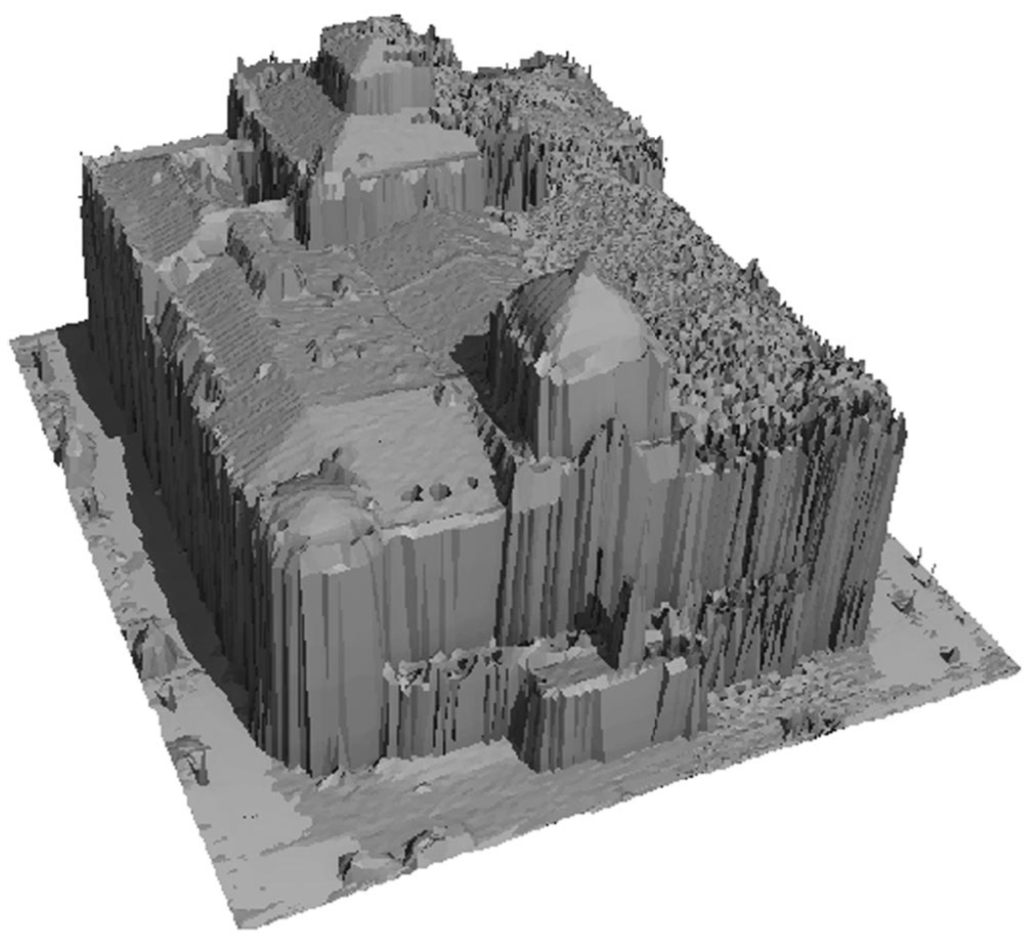
\includegraphics[width=\linewidth]{figs/data-driven.png}
		\caption{Reconstruction based on a triangulation of the input points \citep{Axelsson99}}%
		\label{subfig:data-driven}
	\end{subfigure}
	\quad
	\begin{subfigure}[b]{0.45\linewidth}
		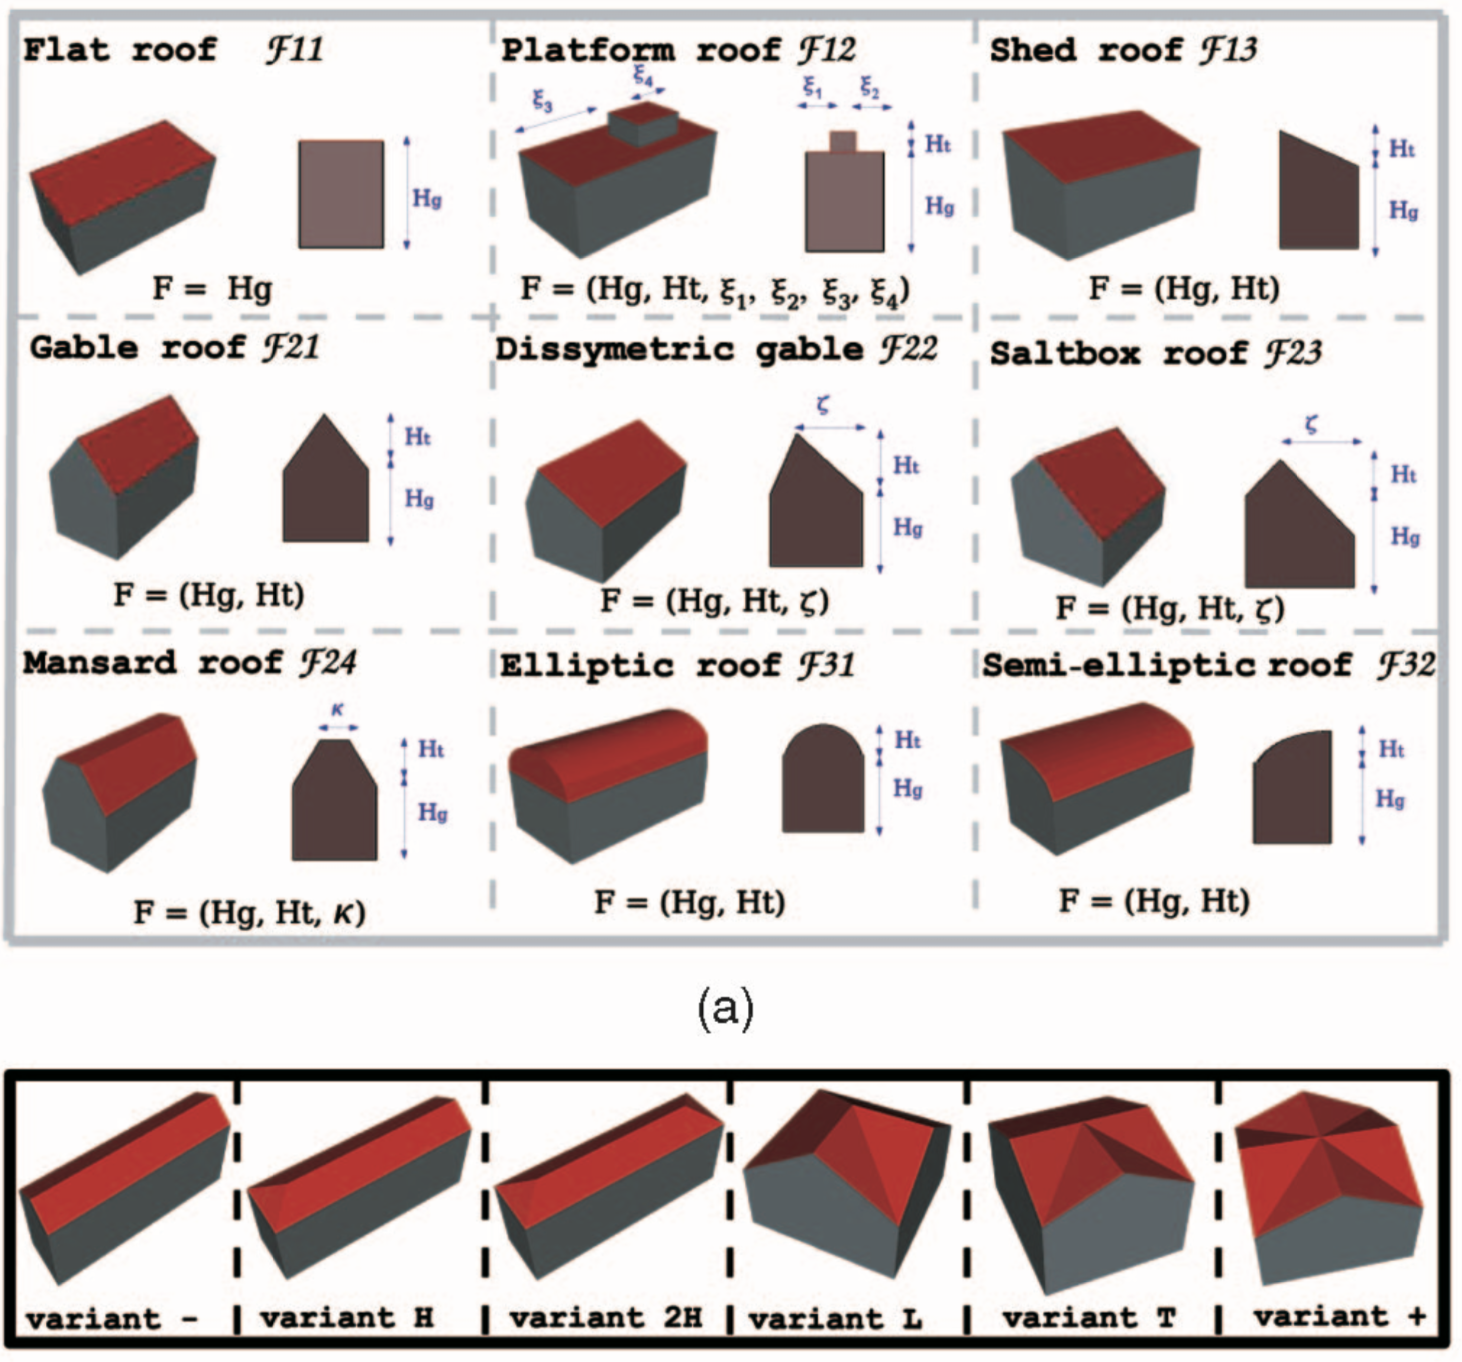
\includegraphics[width=\linewidth]{figs/model-driven.png}
		\caption{Reconstruction by fitting parametrised roof models \citep{Lafarge10}}%
		\label{subfig:model-driven}
	\end{subfigure}
	\caption{Data driven (\subref{subfig:data-driven}) versus model driven reconstruction (\subref{subfig:model-driven})}%
	\label{fig:data-vs-model-driven}
\end{figure}

The data driven approach strongly relies on the quality and completeness of the input data.
The resulting building models have a good data fit, but a high complexity (high number of faces).
Defects in the input data may lead to problems in the building model, such as holes and non-2-manifoldness.
Examples of the data driven approach are methods that triangulate directly the input point cloud (see Figure~\ref{subfig:data-driven}).

The model driven approach, on the other hand, rely on strong modelling assumptions about the building shape.
This typically results in models with a low complexity, but a poorer fit with the input points when compared to a purely data driven approach.
Because the model driven approach does not rely so heavily on the quality of the input, defects in the input point cloud are less likely to lead to problems in the building model.
Examples of the model driven approach are methods that fit a pre-defined roof shapes such as a simple gable roof to a point cloud (see Figure~\ref{subfig:data-driven}). 
Such a method will only work for buildings for which a pre-defined roof shape is available.
Yet, if this the case it can already work reliably for a very sparse point cloud.

Table~\ref{tab:data-vs-model-driven} gives an overview of the various trade-offs between the data driven and the model driven approach. 
\begin{table}[]
	\centering
	\begin{tabular}{p{7cm}|p{7cm}}
	Data driven & Model driven \\
	\hline
	Requires high quality input	& Suitable for low quality input \\
	Good data fit	& Possibly loose data fit \\
	Sensitive to defects in input data &  Can overcome input defects to some extent \\
	High mode complexity & Low model complexity \\
	No assumptions on building shape	&  Strong assumptions on building shape\\
	Can deal with large variety of building shapes	& Limited to specific building shapes\\
	No semantics (\ie\ no distinction roof, wall and floor faces) & Has semantics
	\end{tabular}
	\caption{Trade-offs in data driven versus model driven reconstruction}%
	\label{tab:data-vs-model-driven}
\end{table}
Notice that this table describes merely the two extremes, and that mixed approaches also exist.
%The important thing is that you learn to understand about the 


%In conclusion, it should be clear that there is no such thing as a perfect . 

% model only superstructures with model-driven approach (iconisation)


\section{Automatic LoD2 reconstruction for the Netherlands}
% design context
In this section we will discuss an automatic LoD2 reconstruction method that is developed at TU Delft to work with Dutch open data\footnote{the AHN3 point cloud and the BAG building footprints}. 
The output of this method should have a good data fit and a low model complexity.
In addition the method aims to guarantee water-tightness, 2-manifoldness, and ISO19107 compliance. 
This means the reconstructed models are suitable for various kinds of environmental simulation applications.

% modelling assumptions
\subsection{Modelling assumptions}
The following assumptions are taken in the reconstruction method. They are deemed reasonable for the Dutch input datasets that the method was designed on, and with these assumption the reconstruction problem is somewhat simplified.

\begin{description}
	\item[piecewise planar] The shape of a building can be adequately approximated using planar faces that are detectable from the point cloud.
	\item[2.5D with vertical walls] The roof of the building is 2.5D and all walls are vertical. This implies the 3D building model can be extruded from a 2D planar partition of the roof. The 2.5D assumption is quite reasonable for airborne point cloud, because each building is only scanned from above anyhow.
	\item[footprints] Apart from a point cloud the method also takes 2D building footprints as input. These are used to crop the point cloud for each building. It is assumed that the footprints are up-to-date and well aligned with the point cloud.
\end{description}

% data or model driven?
The method can be classified as a mix between the purely data and model driven approaches as discussed in the previous section. 
Consequently it also mixes the benefits and trade-offs of both extremes.
For example, instead of forcing complete roof shapes on a point cloud, it is assumed a building is composed of planar surfaces.
This makes the method more flexible compared to a purely data driven approach that fits a pre-defined roof shape, since it should be able to handle any possible roof shape that consists of planar surfaces.
However, roofs with non-planar surfaces such as spheres could lead to problems.
Therefore the model is not quite as flexible as the more data-driven approaches.


% overview method
\subsection{Method overview}
The method roughly consists of two parts.
In the first part the input footprint partitioned into roof parts.
And in the second part this 2D roof partition is extruded into a 3D model.

%The method consists of five steps.
%\begin{enumerate}
%	\item Plane detection
%	\item Line detection and regularisation
%	\item Subdivision of the footprint
%	\item Graph-cut optimisation
%	\item Extrusion
%\end{enumerate}

%\paragraph{Plane detection} 
\subsubsection{Footprint partitioning}
\begin{myfloat}
	\begin{link-box}
		The reader is advised to read the section on shape detection in the Chapter \emph{Point cloud processing} in the book \href{https://github.com/tudelft3d/terrainbook/releases}{\emph{Computational modelling of terrains}}.
	\end{link-box}
\end{myfloat}
The input footprint is partitioned using lines that are derived from roof planes that are detected in the building point cloud.
The roof planes are detected using a region-growing algorithm and then two type of lines are derived from the planes: boundary lines and intersection lines (see Figure~\ref{subfig:shapedetection}).
\begin{figure}
	\centering
	\begin{subfigure}[b]{0.3\linewidth}
		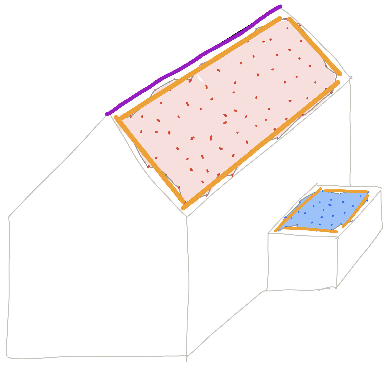
\includegraphics[width=\linewidth]{figs/shapedetection.pdf}
		\caption{Line detection}%
		\label{subfig:shapedetection}
	\end{subfigure}
	\quad
	\begin{subfigure}[b]{0.58\linewidth}
		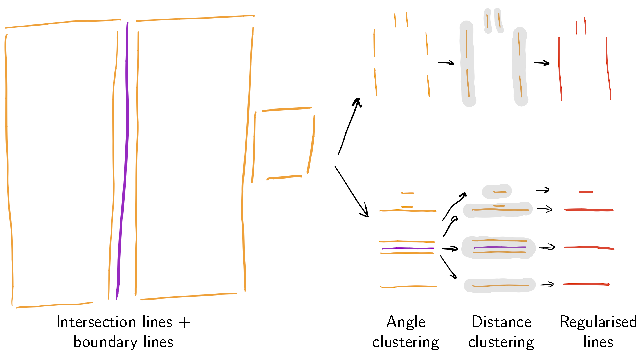
\includegraphics[width=\linewidth]{figs/regularisation.pdf}
		\caption{Line regularisation}%
		\label{subfig:regularisation}
	\end{subfigure}
	\caption{Line detection and regularisation. Boundary lines in orange, intersection lines in purple.}%
	\label{fig:lines}
\end{figure}
The boundary lines are created by detecting lines in the boundary of the $\alpha$-shape of each detected roof plane.
The intersection lines are created where adjacent planes intersect, \eg\ on the top of the gable roof in Figure\ref{subfig:shapedetection}.

Before the boundary and intersection lines are used to subdivide the footprint, they are regularised.
The goal of line regularisation is to remove duplicate lines.
For example, the line on top of the gable roof in Figure~\ref{subfig:shapedetection} is detected three times: once as an intersection line and twice as a boundary line (once for each incident roof plane).
After line regularisation only a single line remains.
Line regularisation is done in two steps: angle clustering and distance clustering (see Figure~\ref{subfig:regularisation}).
Angle clustering is performed first, and in this step lines that have approximately the same orientation in the 2D plane are put in the same angle cluster.
In distance clustering the angle clusters are further divided into distance clusters.
This is done by computing for each angle cluster the distances between the lines it contains.
Groups of lines with a small distance with respect to each other are put in a separate distance cluster.
Finally, one representative line is selected for each distance cluster.

After the lines are detected and regularised they are used to subdivide the footprint into a planar partition (first operation in Figure~\ref{fig:roofpartition}).
\begin{figure}
	\centering
	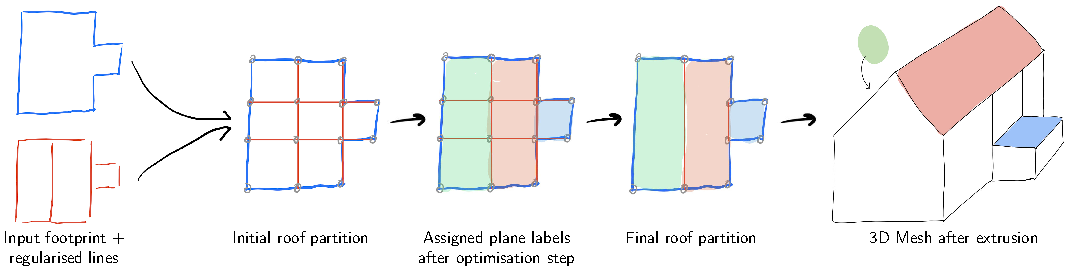
\includegraphics[width=\linewidth]{figs/roofpartition.pdf}
	\caption{Operations on the roof partition}%
	\label{fig:roofpartition}
\end{figure}
A doubly connected edge list (DCEL) is used to represents the full topology of the planar partition of the footprint, that is referred to as the \emph{initial roof partition}.
This means that each intersection is explicitly represented with a vertex.
In addition there are no dangling edges.
The use of a DCEL allows for easy traversal and manipulation of the roof partition, \eg\ for the extrusion to a 3D mesh in the last step.


Depending on the number of lines that remain after regularisation, the initial roof partition may have a high complexity; it may contain many small faces.
To reduce the complexity of the roof partition, an optimisation step is performed\footnote{Graph-cut optimisation is used. The details on how graph-cut optimisation works are outside the scope of this course.}.
In this step a roof plane is assigned to each face in the roof partition (second operation Figure~\ref{fig:roofpartition}).
This is done in such a way that 1) the total error with the input point cloud is minimised and 2) the total length of the edges between faces of a different roof plane is minimised.
This  optimisation thus seeks an optimal balance between respectively a good data fit and a low complexity of the roof partition.
After the optimisation is complete, the edges for which the two incident faces are assigned to the same roof plane are removed from the partition (third step Figure~\ref{fig:roofpartition}).
The faces in the resulting \emph{final roof partition} are referred to as \emph{roof parts}.

\subsubsection{Extrusion}
\label{sec:extrusion}
The final roof partition is transformed into a 3D building mesh using extrusion (fourth step Figure~\ref{fig:roofpartition}).
This is done by exploiting the topological information that is available in the the DCEL of the roof partition, as illustrated in Figure~\ref{fig:extrusion}.
\begin{figure}
	\centering
	\begin{subfigure}[b]{0.4\linewidth}
		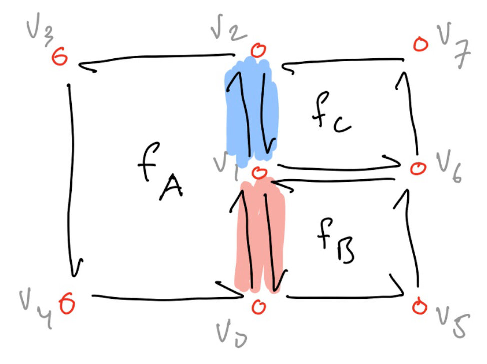
\includegraphics[width=\linewidth]{figs/2DDCEL.pdf}
		\caption{2D roof partition as a DCEL}%
		\label{subfig:2ddcel}
	\end{subfigure}
	\quad
	\begin{subfigure}[b]{0.3\linewidth}
		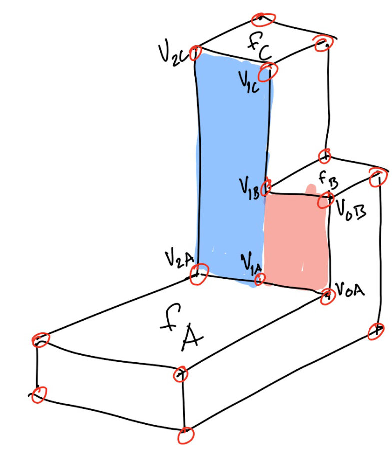
\includegraphics[width=\linewidth]{figs/3DDCEL.pdf}
		\caption{Extruded 3D mesh}%
		\label{subfig:3ddcel}
	\end{subfigure}
	\caption{Extrusion from the roof partition}%
	\label{fig:extrusion}
\end{figure}
Notice that the building mesh consists of three types of faces, \ie\ the floor, the roof and the wall faces.
These are generated from the roof partition in separate procedures.

\begin{description}
\item[floor face] The geometry of the floor face consists of the edges in the roof partition that are incident to the exterior to the footprint. The elevation of the floor face can either be set to the lowest ground point around the building, or if a terrain mesh is available it can be made exactly fitting with the terrain by computing the intersection with that terrain mesh and setting the vertex elevations accordingly.

\item[wall faces] These are vertical faces that connect the floor face with the roof faces. They are extruded from the edges in the roof partition that have two incident roof parts. Depending on the plane configuration of the incident roof parts an edge is extruded differently. Figure~\ref{fig:extrusion-edge:cases} shows a few possible cases (there are more).
\begin{figure}
	\centering
	\begin{subfigure}[b]{0.25\linewidth}
		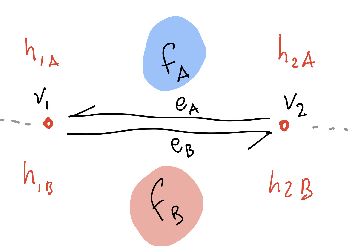
\includegraphics[width=\linewidth]{figs/extrusion-edge.pdf}
		\caption{Edge $e$ in the roof partition with its incident roof parts}%
		\label{fig:extrusion-edge:detail}
	\end{subfigure}
	\quad
	\begin{subfigure}[b]{0.7\linewidth}
		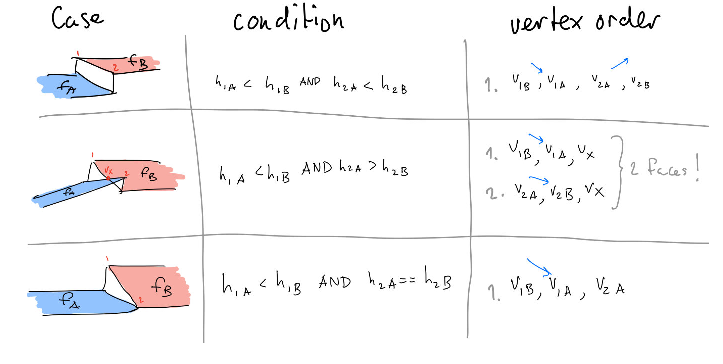
\includegraphics[width=\linewidth]{figs/extrusion-edge-cases.pdf}
		\caption{Various possible roof face configurations at edge $e$}%
		\label{fig:extrusion-edge:cases}
	\end{subfigure}
	\caption{Determining wall face geometry and orientation. $h_{1A}$ denotes the elevation at vertex $v_1$ on face $f_A$.}%
	\label{fig:extrusion-edge}
\end{figure}
Notice that an edge can generate 0 (if the incident plane intersect exactly at the edge), 1 or 2 wall faces.
Also notice that the order of the vertices of a wall face (so that they are oriented counter-clockwise around the face normal that points to the exterior of the mesh) is completely determined by the plane configuration case at the edge.

Special attention needs to be paid to vertices that are extruded to more than two elevations such as $v_1$ in Figure~\ref{fig:extrusion}.
To get a topologically correct building mesh, the extruded vertices should become part of all their incident wall faces.
Vertex $v_{1B}$ should thus also be inserted in the boundary ring of the blue face in Figure~\ref{subfig:3ddcel}, despite the fact it is co-linear with $v_{1A}$ and $v_{1C}$.

\item[roof faces]  Each roof part in the interior of the roof partition will generate a roof face in the building mesh. The planimetric geometry of the roof faces is identical to the faces in the roof partition. The vertex elevations are found by projecting the 2D vertices to the plane of the roof part.
\end{description}

%%%
%
%\section{Notes and comments}
% TODO : complete notes



%%%
%
\section{Exercises}

\begin{enumerate}
  \item Explain the advantages of 2-manifoldness in a building model
  \item Complete the table of possible plane configurations in Figure~\ref{fig:extrusion-edge:cases}.
  \item Could a non-manifold edge be created in the extrusion that is described in Section~\ref{sec:extrusion}? If so, describe how that could happen.
\end{enumerate}



%-------------------------------------------
%-- References
%-------------------------------------------
\bibliographystyle{../../refs/geo1004}
\bibliography{../../refs/geo1004}

\end{document}

